% \s{ハミルトニアン} \label{sec:form:hami}

次のハミルトニアンで表される、2 成分フェルミ原子気体を考える。
\beq
\hanaH &= \Hkin + \Hint + \Himp.\label{eq:form:ham:total}
\eeq
ここで、$\Hkin$ は自由フェルミ原子の運動エネルギー項、$\Hint$ はフェルミ間の接触型引力相互作用、そして $\Himp$ は非磁性不純物を表す。以下、これら各項について説明する。

先ず、運動エネルギー項 $\Hkin$ は第 2 量子化表示で次式で与えられる。
\beq
&\Hkin =  \sum_{\bp, \spin} \left( \ken_{\bp} - \cpt \right) c_{\bp \spin}^{\dag} c_{\bp \spin}. \label{eq:form:ham:hkin}
\eeq
ここで、$c_{\bp \spin}$ は運動量 $\bp$、(クーパー対形成に関与する 2 つの超微細構造状態を表す)擬スピン $\spin = \uar, \dar$ のフェルミ原子の消滅演算子を表す。$\ken_{\bp} = \bp^2 / (2m)$ はフェルミ原子の運動エネルギーで $m$ は原子の質量である。$\cpt$ は化学ポテンシャルである。


フェルミ原子間にはたらく引力相互作用を表す $\Hint$ は、
\beq
&\Hint = - \uint \sum_{\bp, \bpp, \bq}c_{\bp+\bqt,\uar}^{\dag} c_{-\bp+\bqt,\dar}^{\dag} c_{-\bpp + \bqt, \dar} c_{\bpp+\bqt, \uar}.\label{eq:form:ham:hint}
\eeq
ここでは接触型相互作用を考えているため、相互作用は逆向きの擬スピン間にのみはたらく。また $U$ は引力相互作用の強度を表す。ここでは $\Lisix$ や $\Kafor$ フェルミ原子気体を考え、$U$ はフェッシュバッハ共鳴により可変であるとする。

式 (\ref{eq:form:ham:total}) の右辺最終項は非磁性不純物散乱を表し、
\beq
&\Himp =  \sum_{i=1}^{\Nimp}\sum_{\bp, \bpp, \spin} e^{i(\bp-\bpp)\cdot \bri} \vimp c_{\bp\spin}^{\dag}c_{\bpp \spin},\label{eq:form:ham:himp}
\eeq
である。ここで、 $\vimp$ は不純物の散乱ポテンシャル、$\Nimp$ は不純物の数、$\bri$ は $i$ 番目の不純物の位置を表す。不純物散乱が擬スピン $\spin$ を変えず、さらに $\spin=\uar, \dar$  に対して同じ強度で散乱することから、非磁性不純物を表していることがわかる。

\ref{sec:form:bcsl} 節では、絶対零度の超流動状態を扱うが、その場合には 2 成分 Nambu 表示を用いるのが便利である。2 成分 Nambu 場、
\beq
\psip = \begin{pmatrix}c_{\bp, \uar}\\ c_{-\bp,\dar}^{\dag}\end{pmatrix},
\eeq
を用い、重要でない定数項を無視すると、式 (\ref{eq:form:ham:hkin}), (\ref{eq:form:ham:hint}), (\ref{eq:form:ham:himp}) の各項はぞれぞれ次のように書き表される:
\beq
&\hkin = \sum_{\bp} \psipd\  \left[ \ken_{\bp}-\cpt \right]\tau_3 \psip,\label{eq:form:ham:shkin}\\
&\hint = -\uint\sum_{\bq}\rho_+(\bq) \rho_-(-\bq) ,\label{eq:form:ham:shint}\\
&\himp = \sum_{i=1}^{\nimp} \sum_{\bp,\bpp} e^{i(\bp-\bpp) \cdot \bri} \psipd \vimp \tau_3 \vpsi_{\bp'}.\label{eq:form:ham:shimp}
\eeq
ここで、
\beq
\tau_1=\begin{pmatrix} 0 & 1 \\ 1 & 0 \end{pmatrix},\ \tau_2=\begin{pmatrix} 0 & -i \\ i & 0 \end{pmatrix}, \ \tau_1=\begin{pmatrix} 1 & 0 \\ 0 & -1 \end{pmatrix},\notag
\eeq
はパウリ行列である。式 (\ref{eq:form:ham:shint}) において、$\rho_s(\bq)$ は一般化された密度演算子であり、次式で与えられる。
\beq
\rho_{\pm} = \sum_{\bp} \varPsi^{\dag}_{\bp} \tau_{\pm} \varPsi_{\bp-\bq}.
\eeq
ここで、
\beq
\tau_+ = \frac{1}{2} \left[ \tau_1 + i \tau_2 \right] = \begin{pmatrix}0& 1 \\ 0& 0\end{pmatrix},\\
\tau_- = \frac{1}{2} \left[ \tau_1 - i \tau_2 \right] = \begin{pmatrix}0& 0 \\ 1& 0\end{pmatrix},
\eeq
を用いた。

\s{フェルミ原子間相互作用 $\Uint$ に対する $s$ 波散乱長 $\as$}\label{sec:form:askfi}


冷却フェルミ原子気体の分野では原子間相互作用の強さは、通常、裸の相互作用 $U$ ではなく、$s$ 波散乱長 $\as$ として測定されるので、理論を構築する際も相互作用強度を $\as$ で与えられるように定式化しておくと、実際と比較する際都合が良い。また、前述したようにフェッシュバッハ共鳴に因る相互作用にはフォノン媒介型相互作用におけるデバイ周波数のような物理的なカットオフがない為、接触型相互作用に起因する紫外発散を除く必要があるが、後述するようにこれをくりこみ処理により散乱長 $\as$ に吸収させることができる。

式 (\ref{eq:form:ham:total}) のハミルトニアンの相互作用 $\Hint$ 中にある裸の相互作用 $U$ と $s$ 波散乱長$ \as$ の関係は次式で与えられる \cite{ohashi2005}。
\beq
\frac{ 4 \pi \as}{m} =  \frac{-\uint}{1 - \uint \sum_{p}^{\omega_c} \frac{1}{2 \ken_p}}.\label{eq:form:ham:askf}
\eeq
ここで $\omega_c$ は形式的に導入したカットオフエネルギーである。相互作用を $\as$ を用いて表すと相図 \ref{fig:bcsbecsouzu}にあるように $\askfi \ltsim -1$ が弱結合 BCS 領域($\tc$ 以下は平均場 BCS 状態に近い)、$\askfi \gtsim +1$ が強結合 BEC 領域($\tc$ 以上でも強い引力相互作用により 2 体束縛状態としての分子ボソンが形成される)となる。$-1 \ltsim \askfi \ltsim 1$ の領域はユニタリ領域、特に $\askfi \to 0\  (\as\to \pm\infty)$ は、ユニタリ極限と呼ばれる。ユニタリ領域は、フェルミ対の形成と解離の繰り返しで特徴付けられる超流動ゆらぎが顕著な領域である。

\s{有限濃度の不純物に対する分布平均と自己無撞着 $T$ 行列近似}\label{sec:form:imp}

式 (\ref{eq:form:ham:himp}) で記述される有限濃度の不純物は特定の不純物配置 $\{\bri\}$ に依存しており系の並進対称性が失われている。特定の不純物配置 $\{\bri\}$ に依存しない結果を得るために、ここでは様々な不純物の分布に関する平均をとる(その結果、理論としては並進対称性が回復する)。不純物の分布平均の取り方には様々な方法があるが、ここでは金属電子系で用いられてきた、自己エネルギーに対する不純物の位置平均を採用する。すなわち与えられた自己エネルギー $\sig^{\imp}_{\bp, \bpp}(i \omn, \bm{R}_1, \bm{R}_2, \dots, \bm{R}_{\nimp})$ に対し(ここで $\omn = \pi T(2 n + 1)$、$n=0, \pm1, \dots$ はフェルミオン松原周波数)、不純物の分布平均をとった自己エネルギー $\sigimppom$ を次式で与える。
\beq
\sigimppom \delta_{\bp,\bpp} = \frac{1}{V^{\nimp}}\int \diff \bm{R}_1 \cdots \diff \bm{R}_{\nimp}  \sig^{\imp}_{\bp, \bpp}(i \omn, \bm{R}_1, \bm{R}_2, \dots, \bm{R}_{\nimp}).
\eeq
ここでは、体積 $V$ を明示した。この方法は、金属超伝導の不純物効果の研究でも用いられている \cite{abrikosov1961,shiba1968, shiba1973}。この操作により並進対称性が回復するので、自己エネルギーは運動量について対角的になる。左辺のクロネッカーデルタ $\delta_{\bp, \bpp}$ はそれを反映したものである。

\begin{figure}[t]
\begin{center}
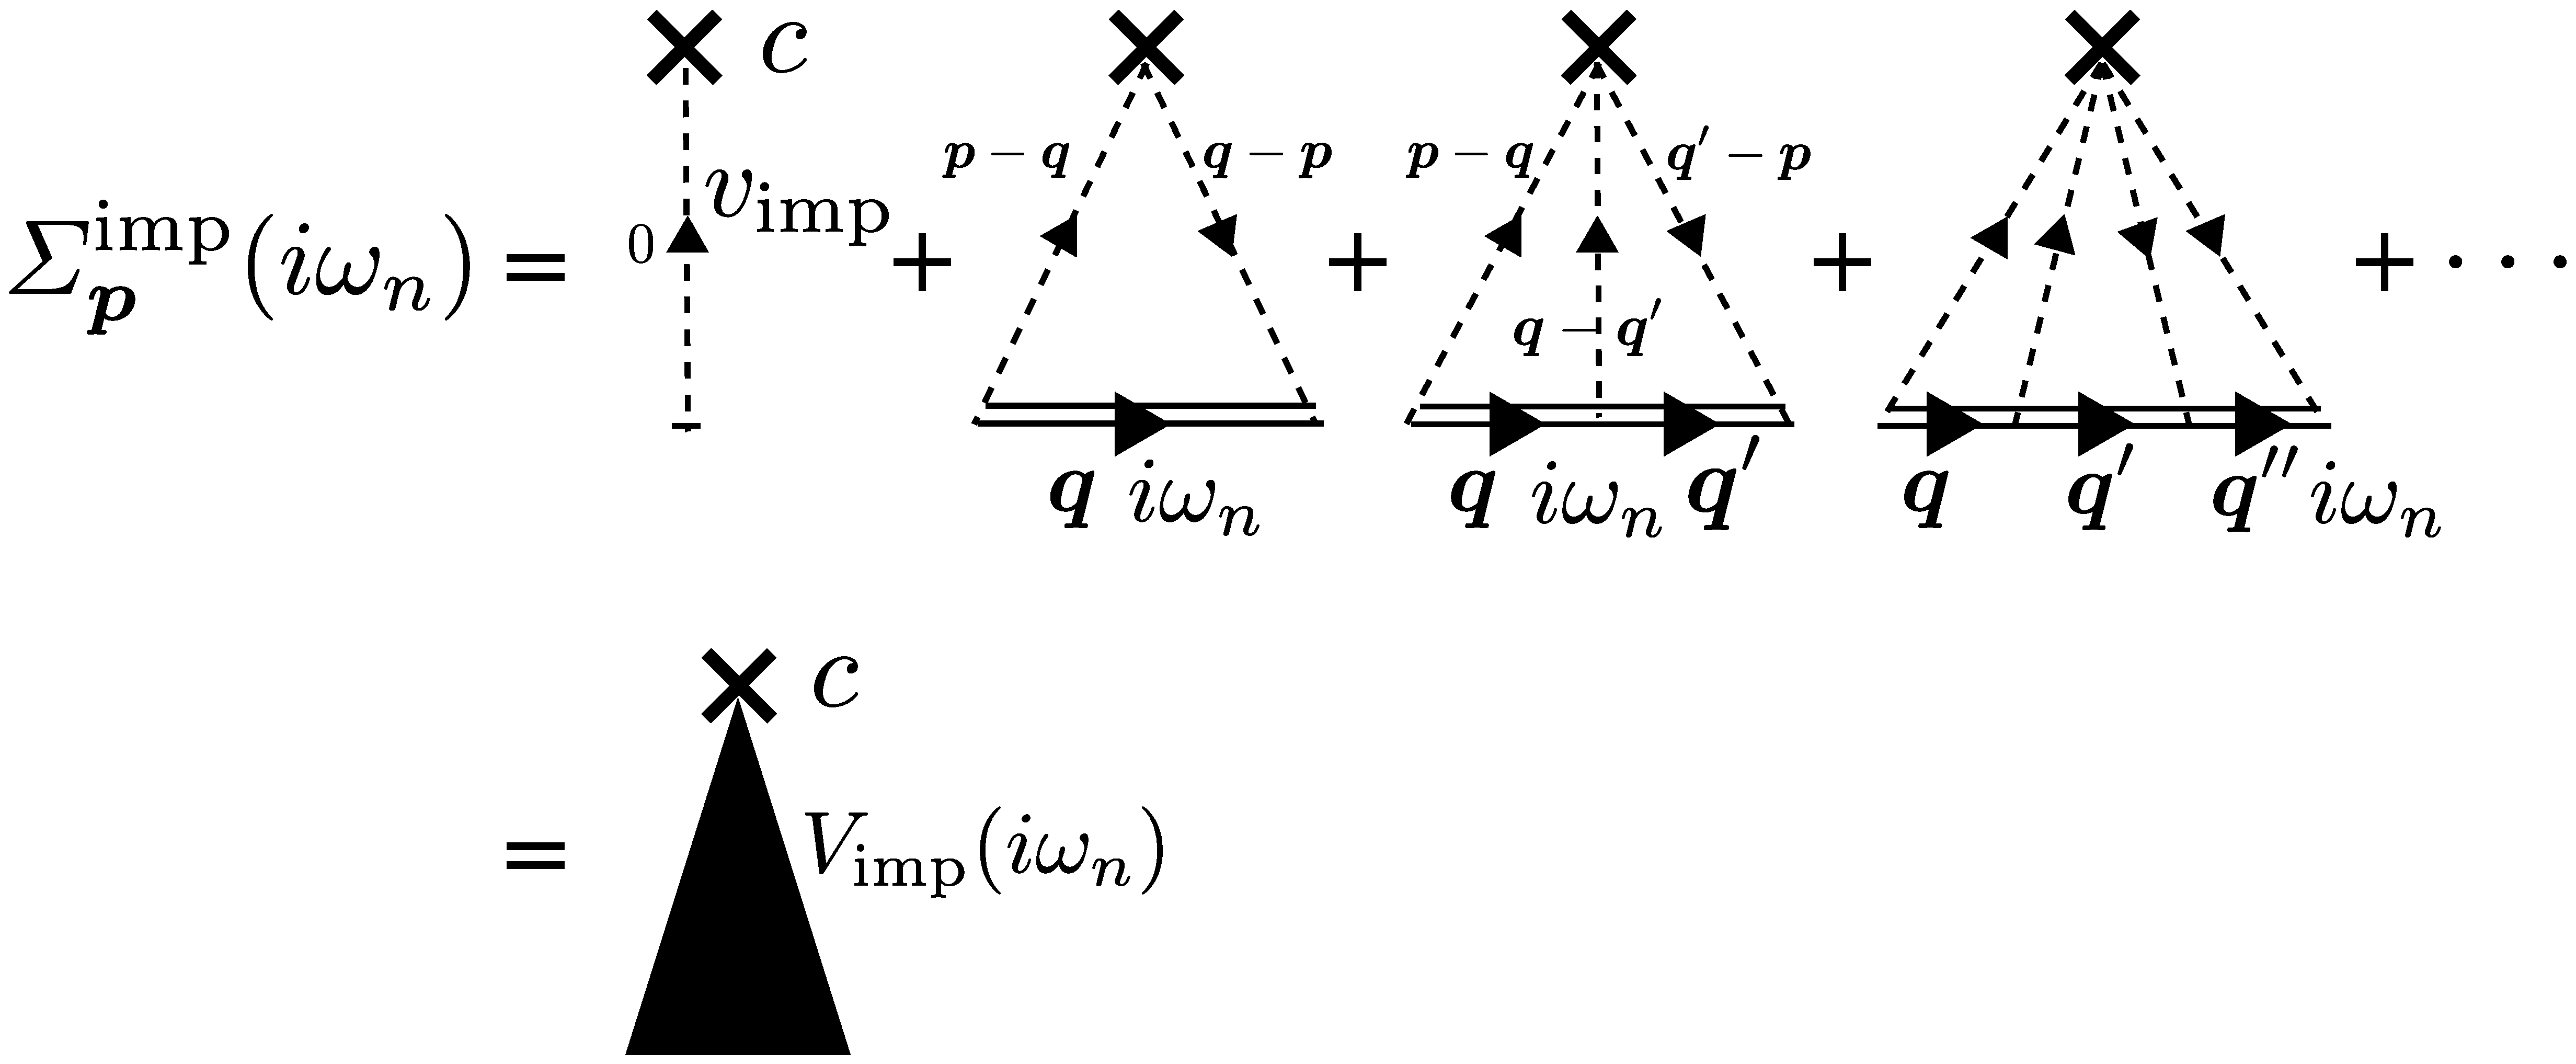
\includegraphics[width=120mm]{eps/sig-impimp.eps}
\end{center}
\caption{非磁性不純物散乱に対する自己無撞着 $T$ 行列近似を表すファインマンダイアグラム。図中、破線は不純物散乱ポテンシャル $\vimp$、二重線は 1 粒子温度グリーン関数 $\gimppom$、$\times$ 印は不純物濃度 $c$ を表す。この近似は、一つの不純物による任意回の不純物散乱を含み、内線も不純物散乱の自己エネルギーを含むグリーン関数 $\gimppom$ が用いられている。これら多重散乱をまとめたものが有効不純物散乱ポテンシャル $\vvtxn$ である。}
\label{fig:form:ham:sigimp}
\end{figure}


不純物散乱 $\Himp$ に対し自己無撞着 $T$ 行列近似を採用する。この近似は図 \ref{fig:form:ham:sigimp} のダイアグラムで表され、分布平均をとった後の系のグリーン関数を $\gimppom$ とすると自己エネルギーは、
\beq
\sigimppom &= \con \vimp \frac{1}{1 - \vimp \sum_{\bq} \gimp_{\bq}(i\omn)}\notag\\
& \equiv \con \vvtxn,\label{eq:form:ham:sctma}
\eeq 
となる。ここで、 $c=\nimp/V$($V$ は体積)は不純物濃度である。式 (\ref{eq:form:ham:sctma}) の $\vvtxn$ は不純物の多重散乱を含む有効不純物散乱ポテンシャルを表し、図 \ref{fig:form:ham:sigimp} の二行目の黒三角形のダイアグラムに対応する。本論文では用いないが、式 (\ref{eq:form:ham:sctma}) 中のグリーン関数 $\gimppom$ を無摂動のグリーン関数、
\beq
\gzrpom = \frac{1}{i \omn - \left[ \varepsilon_{\bp}- \cpt\right]},
\eeq
で置き換えたものは $T$ 行列近似と呼ばれる。

不純物濃度は体積濃度、
\beq
c = \frac{\nimp}{V},\label{eq:form:ham:cvolume}
\eeq
として定義されているので、ダイアグラム法を用いる際には図 \ref{fig:form:ham:sigimp} 中の $\times$ 印に $c$ を割り当てれば良い。本論文では $V=1$ としているため、式 (\ref{eq:form:ham:cvolume}) の $c$ は無次元量であるが、計算結果に対し議論をする際にはフェルミ原子数 $N$ で規格化した濃度、
\beq
\overline{c}=\frac{\nimp}{N} = \frac{4}{3} \frac{c}{\fdos \eqf},\label{eq:form:ham:overlinec}
\eeq
を用いると便利である。ここで $\eqf = \kf^2/(2m)$ はフェルミエネルギーであり、
\beq
\fdos = \frac{mk_{\text{F}}}{2\pi^2},
\eeq
は自由フェルミ気体のフェルミ面における 1 粒子状態密度である。

今考えているモデルでは、不純物散乱も式 (\ref{eq:form:ham:himp}) から分かるように接触型を仮定しているので、式 (\ref{eq:form:ham:sctma}) は紫外発散を含む。そこでこれを除去するために不純物散乱ポテンシャル $\vimp$ に対する $s$ 波散乱長 $\bs$ を導入し、引力相互作用の時と同様、紫外発散を $\bs$ にくりこむ。散乱長 $\bs$ は“裸”の不純物散乱ポテンシャル $\vimp$ と次式で関係付けられる:
 \beq
 \frac{2 \pi \bs}{m} = \frac{\vimp}{1-\vimp\sum_p^{\omega_c'} \frac{1}{ \ken_{\bp}}}.\label{eq:form:ham:bskf}
\eeq
ここで、$\omega_c'$ は形式的に導入したエネルギーカットオフである。散乱長 $\bs$ を用いると式 (\ref{eq:form:ham:sctma}) の自己エネルギーは、
\beq
\sigimppom = c\frac{1}{\frac{m}{2\pi \bs} - \sum_{\bq} \left[ \gimp_{\bq}(i\omn) + \frac{1}{ \ken_{\bq}} \right]},\label{eq:form:ham:sctmabs}
\eeq
となり、式 (\ref{eq:form:ham:sctma}) の分母の運動量和が持っていた紫外発散は $\bs$ に吸収されて式 (\ref{eq:form:ham:sctmabs}) からは除かれる(式 (\ref{eq:form:ham:sctmabs})の分母の $\bq$ の和は紫外発散しないことに注意)。

式 (\ref{eq:form:ham:sctma}) において、分母を陽に現れている $\vimp$ に対し 2 次まで展開した上で、 1 次の定数項 $c \vimp$ は定数シフトとして $\cpt$ に吸収させて無視したもの、
\beq
\varSigma^{\text{Born}}_{\text{imp}} ( i \omn) &= c \vimp^2 \sum_{\bq} \gimp_{\bq}(i\omn) = c \left[\frac{1}{\frac{m}{2 \pi \bs} - \sum_{\bq}^{\omega_c}\frac{1}{\ken_{\bq}}}\right]^2 \sum_{\bq} \gimp_{\bq}(i\omn) ,\label{eq:form:ham:scborn}
\eeq 
は自己無撞着ボルン近似と呼ばれ、化学ポテンシャルシフト以上の効果を与える最低次のみを取り出した近似として金属超伝導体に対する不純物効果の研究でよく用いられている。しかし、フェルミ原子気体の場合には、式 (\ref{eq:form:ham:scborn}) を用いると $\bs$ を導入しても物理的なカットオフが存在しないため、非物理的なカットオフに顕わに依存した表式となってしまう。このため、本研究では自己無撞着ボルン近似は用いない。

最後に、不純物散乱に対する自己無撞着 $T$ 行列近似を超伝導状態で考える際に便利な Nambu 表示での表式について説明する。式 (\ref{eq:form:ham:shkin})-(\ref{eq:form:ham:shimp}) のように Nambu 表示すると、不純物散乱には $\tau_3$ が掛かる。結果、Nambu 表示の下での自己エネルギー $\bsigimppom$ は、
\beq
\bsigimppom &= \con \bvvtxn=\con \frac{1}{\frac{m}{2\pi \bs}\tau_3 - \sum_{\bq} \left[ \bgimp_{\bq}(i\omn) + \frac{\tau_3}{ \ken_{\bq}} \right]},\label{eq:form:ham:abcslimp}
\eeq 
となる。ここで、
\beq
\bgimp_{\bp}(i\omn) = \frac{1}{i \omn - \left[\ken_{\bp} - \cpt\right]\tau_3 - \bsigimppom},
\eeq
は2 成分 Nambu 場を用いた $2 \times 2$ 行列の 1 粒子温度グリーン関数である。
%%%%%%%%%%%%%%%%%%%%%%%%%%%%%%%%%%%%%%%%%%%%%%%%%%%%%%%%%%%%